O rok młodszy od stryja Józefa -- \textbf{Karol przyszedł na świat 29 października 1909~r. w Łagiewnikach Wielkich}.

\begin{figure}[!h]
\begin{center}
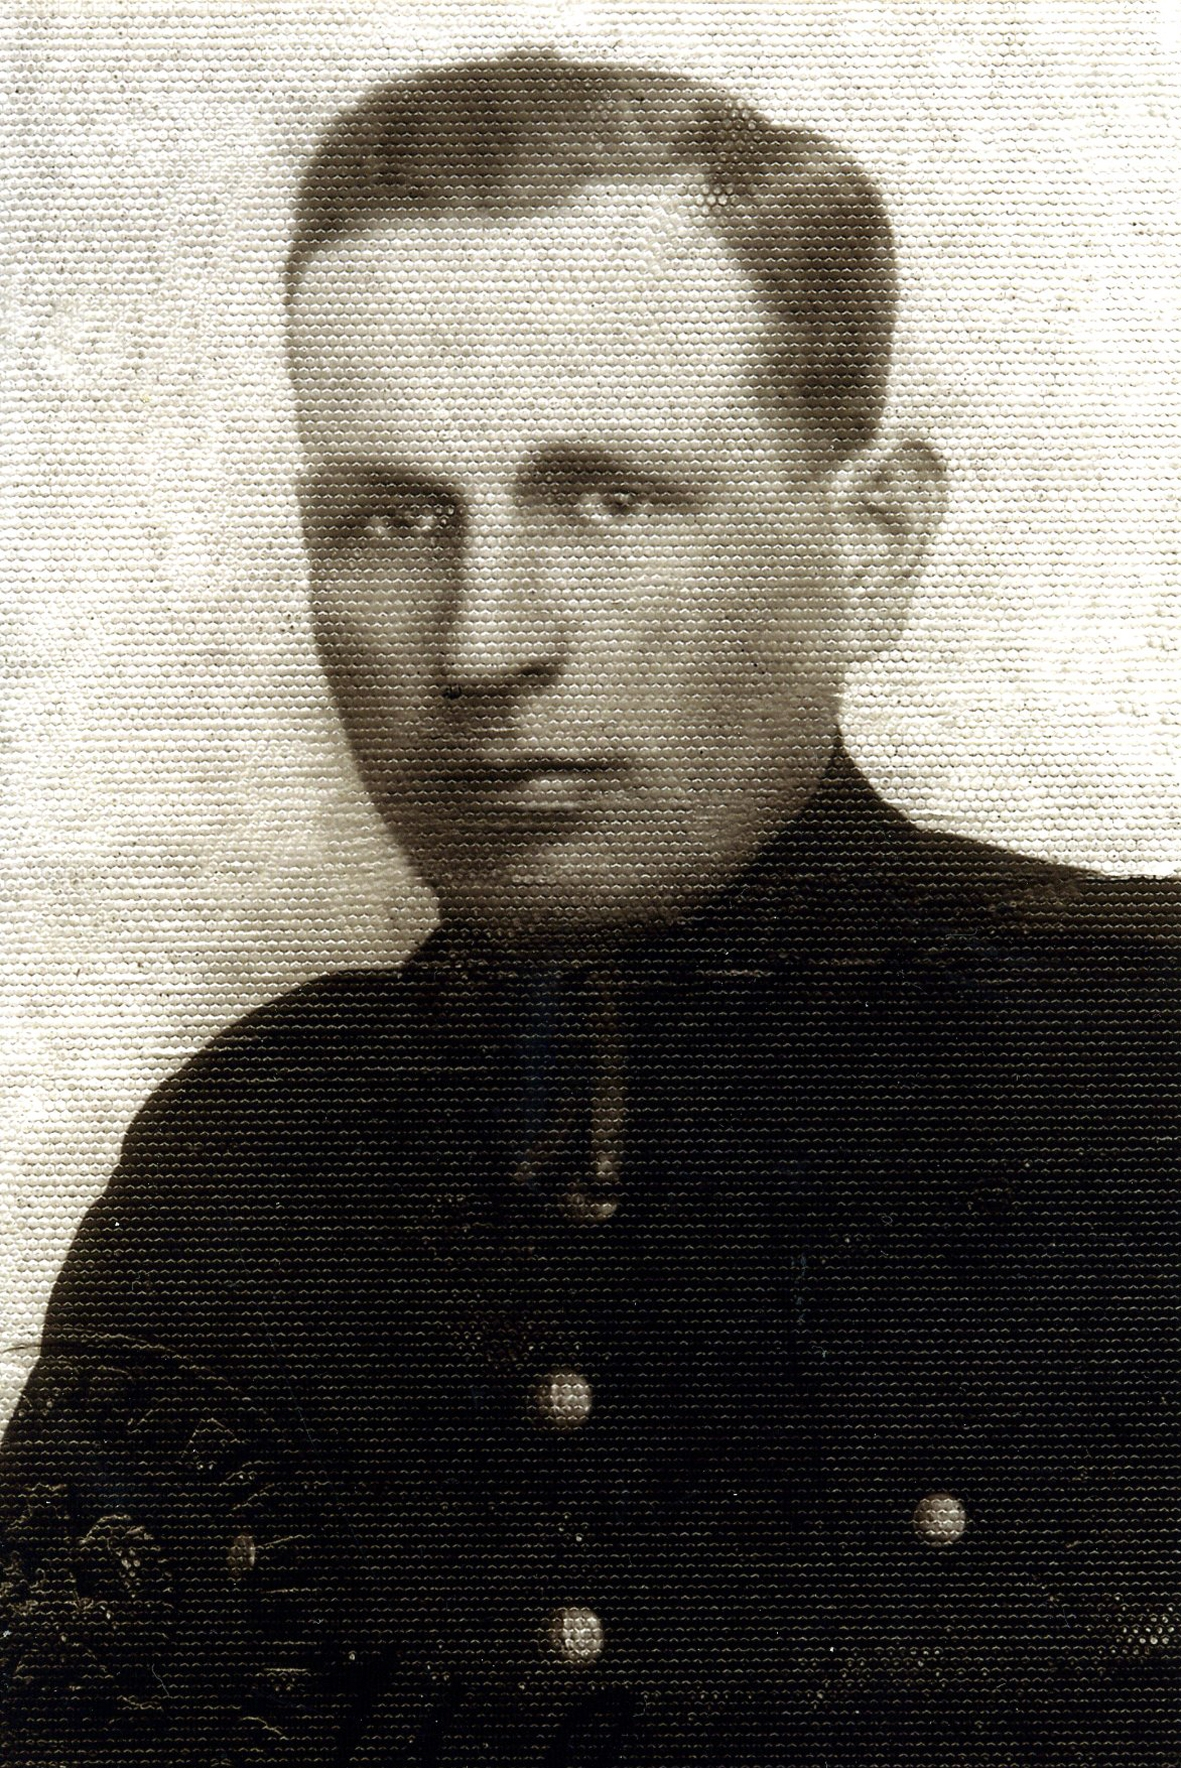
\includegraphics[width=0.2\textwidth]{photo/karol_swierczynski_1.jpg}
\caption{Karol Świerczyński na zdjęciu legitymacyjnym}
\label{rys:karol_swierczynski_1}
\end{center}
\end{figure}

Ukończył on dwuletnią Szkołę Rolniczą w Tarnowskich Górach (zarówno Świerczyńscy jak i Grabińscy cenili sobie wykształcenie dlatego posyłali chłopców, a nawet dziewczyny do szkół) i podjął pracę w folwarku w Jaćmierzu koło Sanoka, a następnie 2 -- 3 lata w Zubrzcu w pow. Buczackim, gdzie pracował aż do powołania go do służby wojskowej w 74 Górnośląskim Pułku, gdzie służył dwa lata. Po wojsku, w którym dosłużył się stopnia kaprala, zaangażował się do pracy w oddziale Więzienia Lublinieckiego -- w Łagiewnikach Wielkich.

\begin{figure}[!h]
\begin{center}
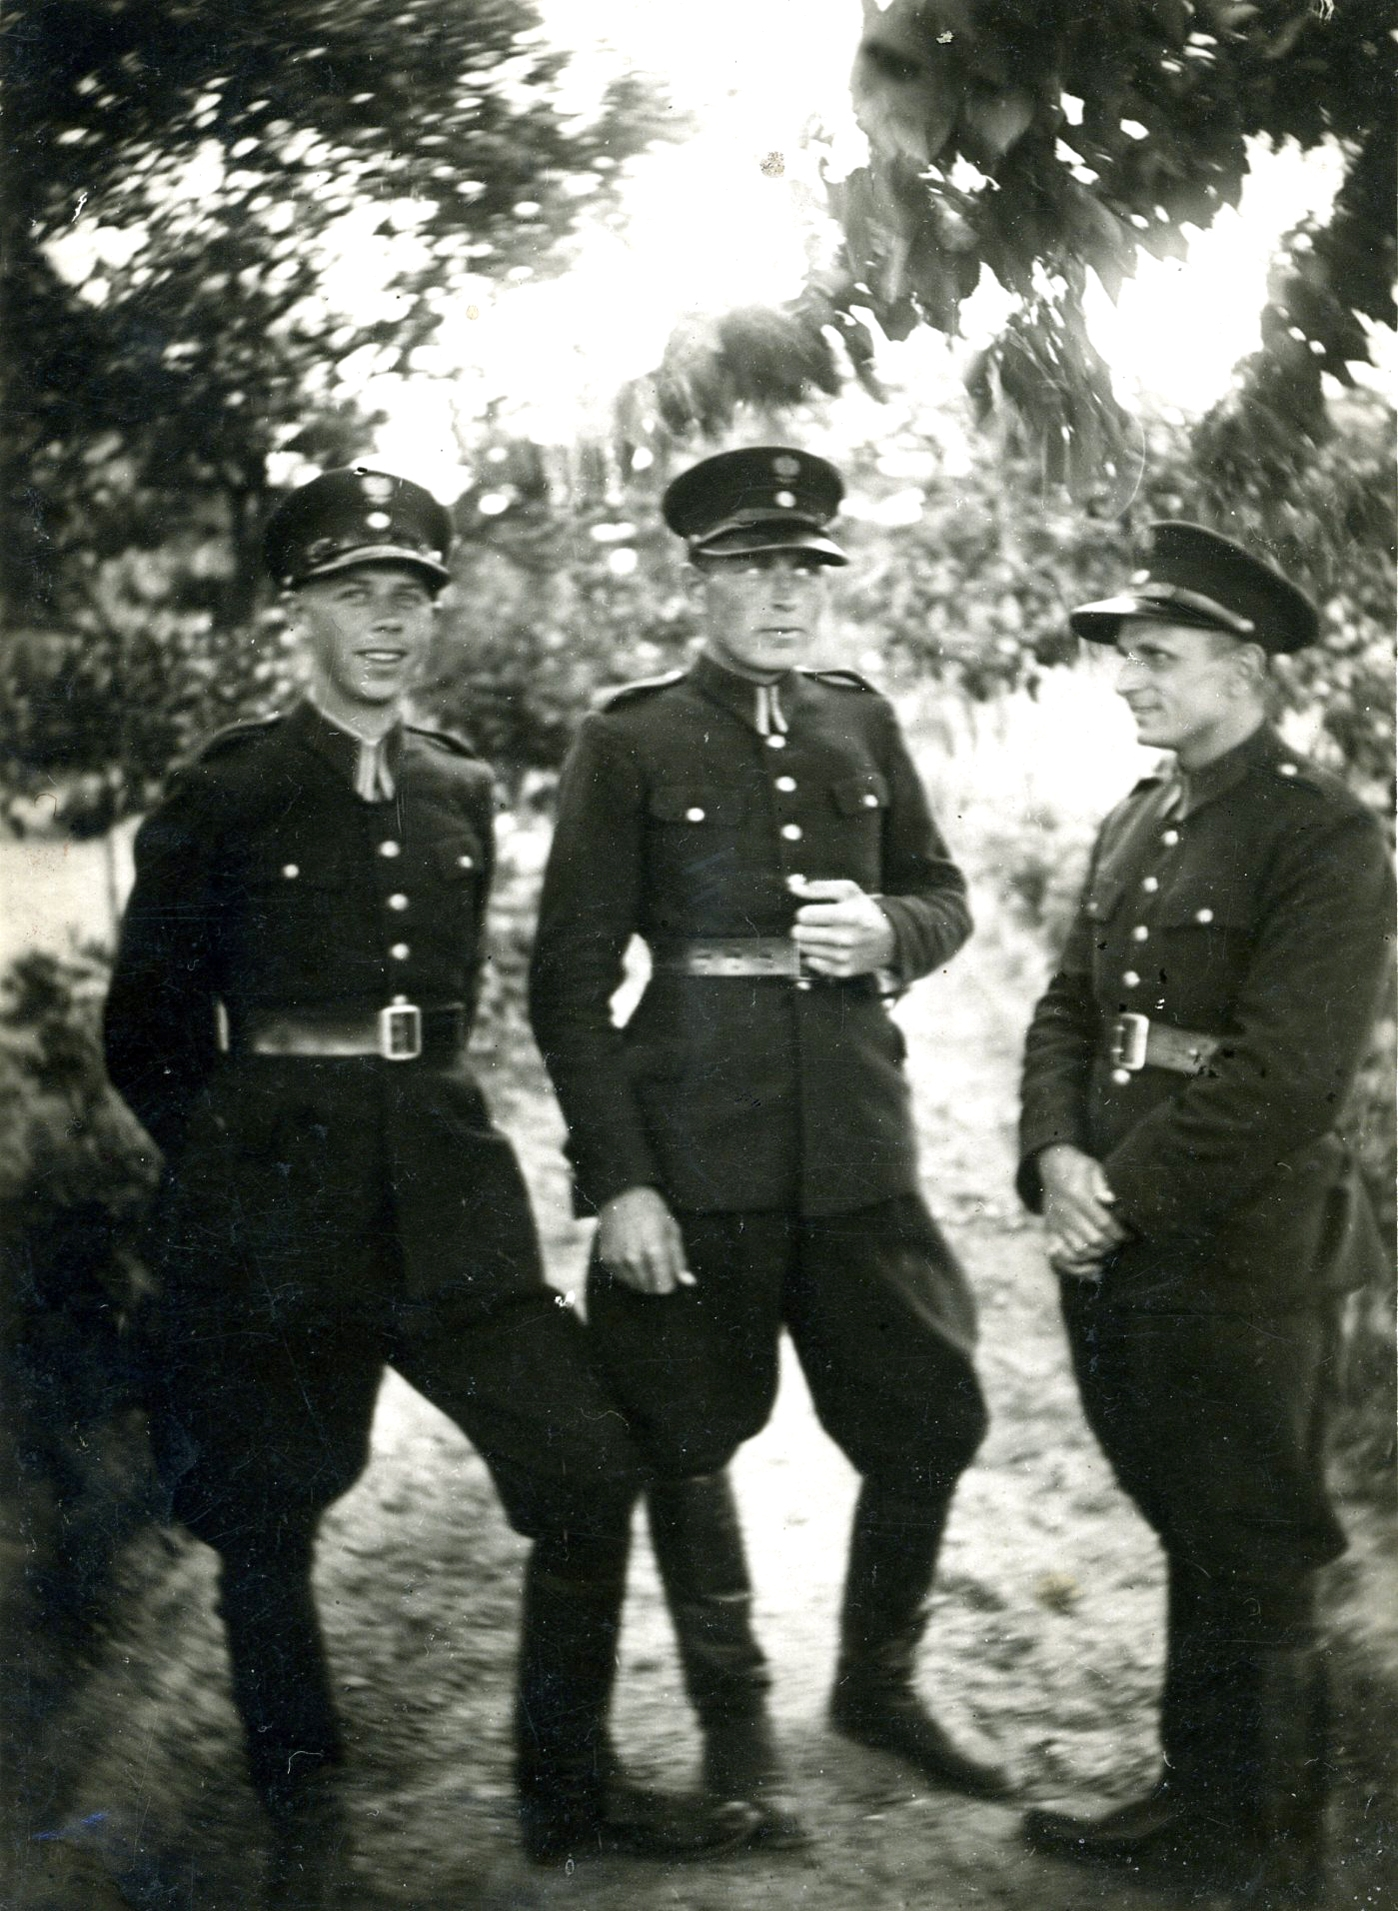
\includegraphics[width=0.35\textwidth]{photo/karol_swierczynski_2.jpg}
\caption[Karol Świerczyński z Antonim Lehmanem]{Na zdj. od lewej NN, Karol Świerczyński w środku z Antonim Lehmanem}
\label{rys:karol_swierczynski_2}
\end{center}
\end{figure}

Tak oto wspomina stryja Karola mój ojciec: \textit{Drugim w kolejności był Karlik. Nie pamiętam, by go ktoś nie lubił. Miał „złote ręce”, uczynny był, pracowity i najmocniejszy z całej rodziny. Gdy pracował w więzieniu, poznał Elżbietę Janik, z którą chodził wiele lat i gdyby nie wojna, pewnie ożeniłby się z nią}.

\begin{figure}[!h]
\begin{center}
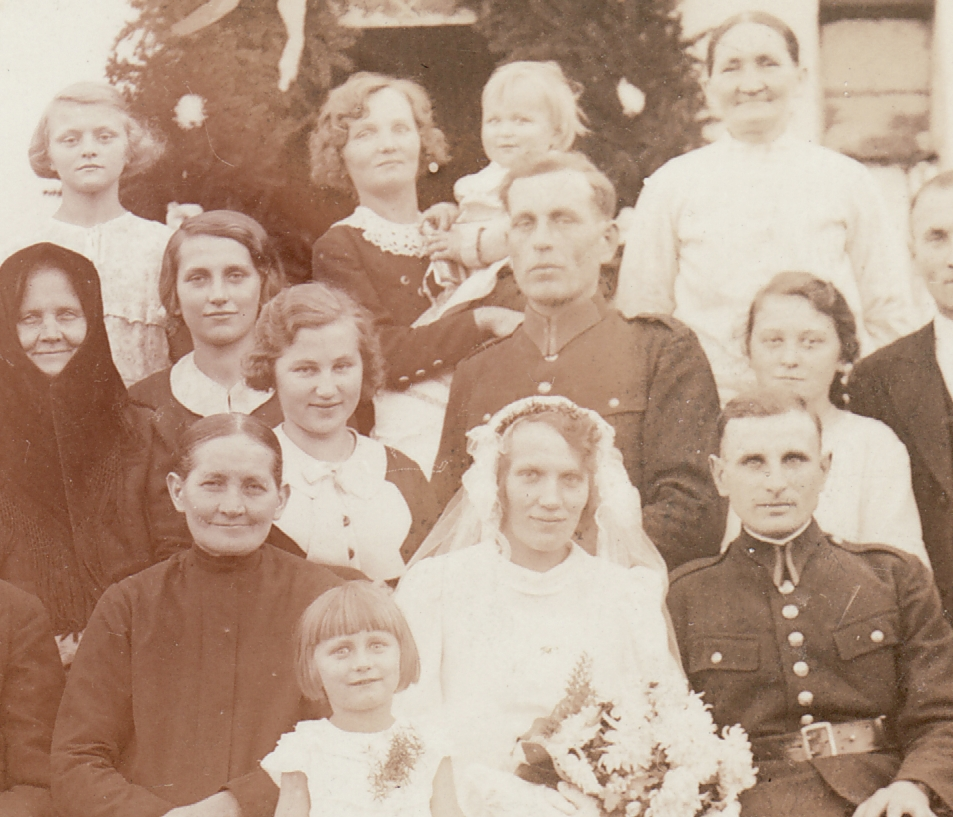
\includegraphics[width=0.5\textwidth]{photo/irena_antoni_lehman_slub_1.jpg}
\caption[Karol Świerczyński i Elżbieta Janik]{Karol Świerczyński i Elżbieta Janik -- stoją razem za stryjenką Ireną i babcią Eufemią (fragment zdjęcia gości weselnych ze ślubu Ireny Świerczyńskiej i Antoniego Lehmana)}
\label{rys:irena_antoni_lehman_slub_1}
\end{center}
\end{figure}

Ona też mu była wierną, przez wiele lat oczekując jego powrotu i nie wychodząc za mąż za kogoś innego.

\begin{figure}[!h]
\begin{center}
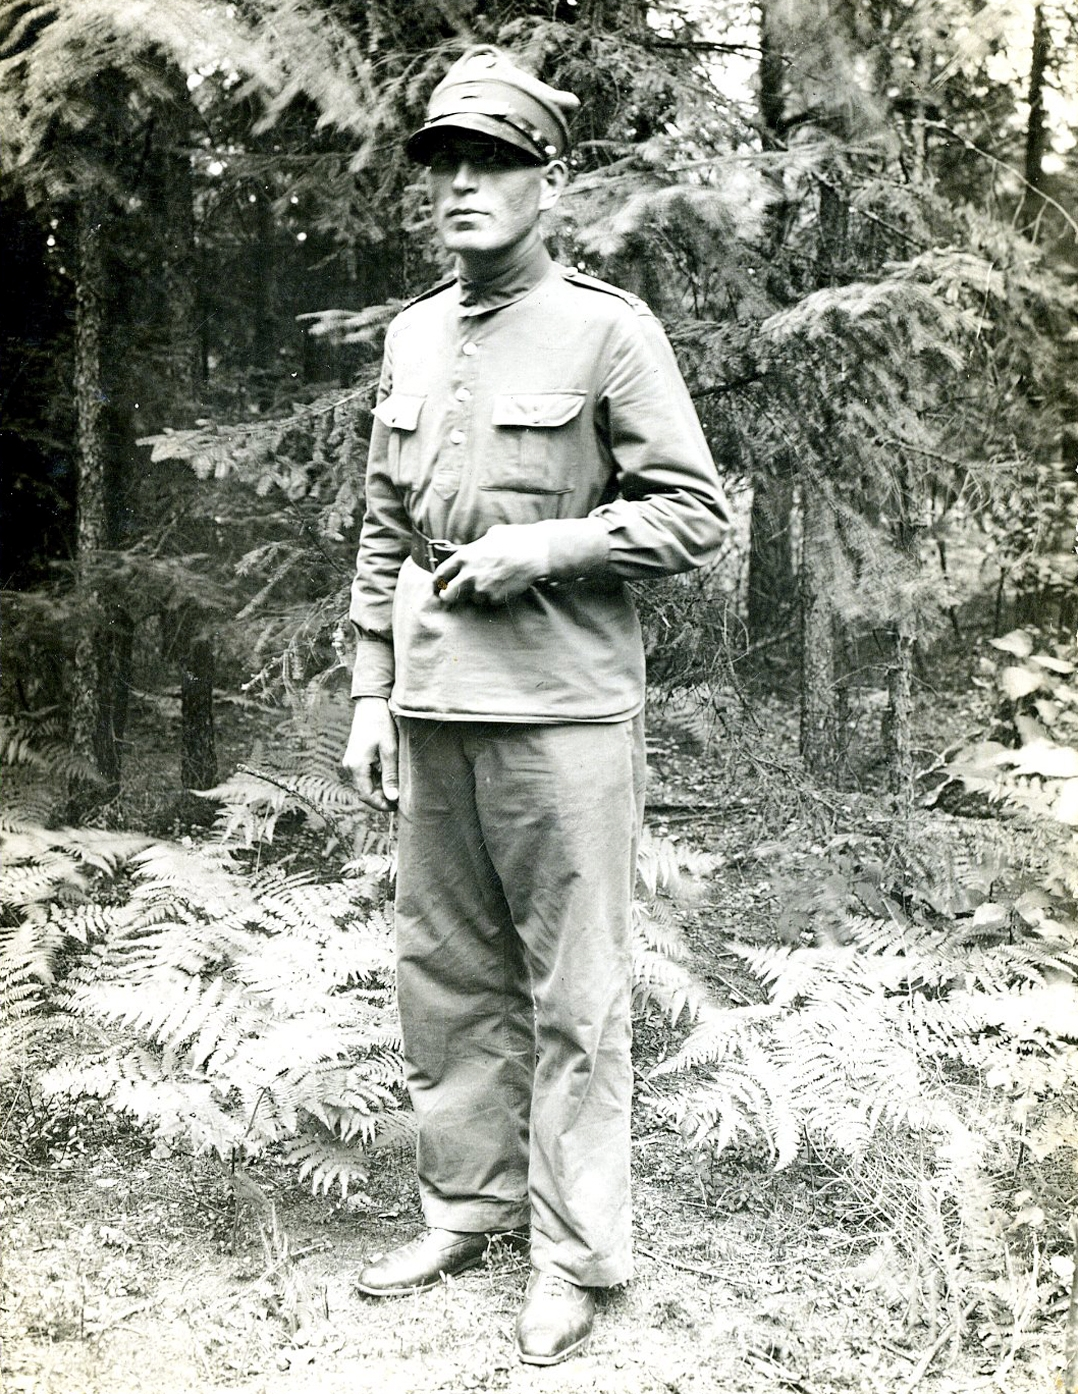
\includegraphics[width=0.4\textwidth]{photo/karol_swierczynski_3.jpg}
\caption{Ostatnie zdjęcie Karola Świerczyńskiego}
\label{rys:karol_swierczynski_3}
\end{center}
\end{figure}

\textbf{Stryj Karol Świerczyński jak tylko został zmobilizowany w ostatnich dniach sierpnia 1939 r. tak po nim słuch zaginął.} Żadnych wieści, a ponieważ archiwa 74 Górnośląskiego Pułku, w którym służył, zostały zniszczone, nie można odnaleźć nawet informacji, w której kompanii, batalionie służył. Zginął może koło Rozprzy, a może w lasach janowskich, a może na Kielecczyźnie, gdzie się wycofywał rozbity pod Janowem pułk? Pewnie nie zginął gdzieś pod Lublińcem – ludziska przecież by swojaka poznali i donieśli rodzinie, że zginął\ldots

\begin{figure}[!h]
\begin{center}
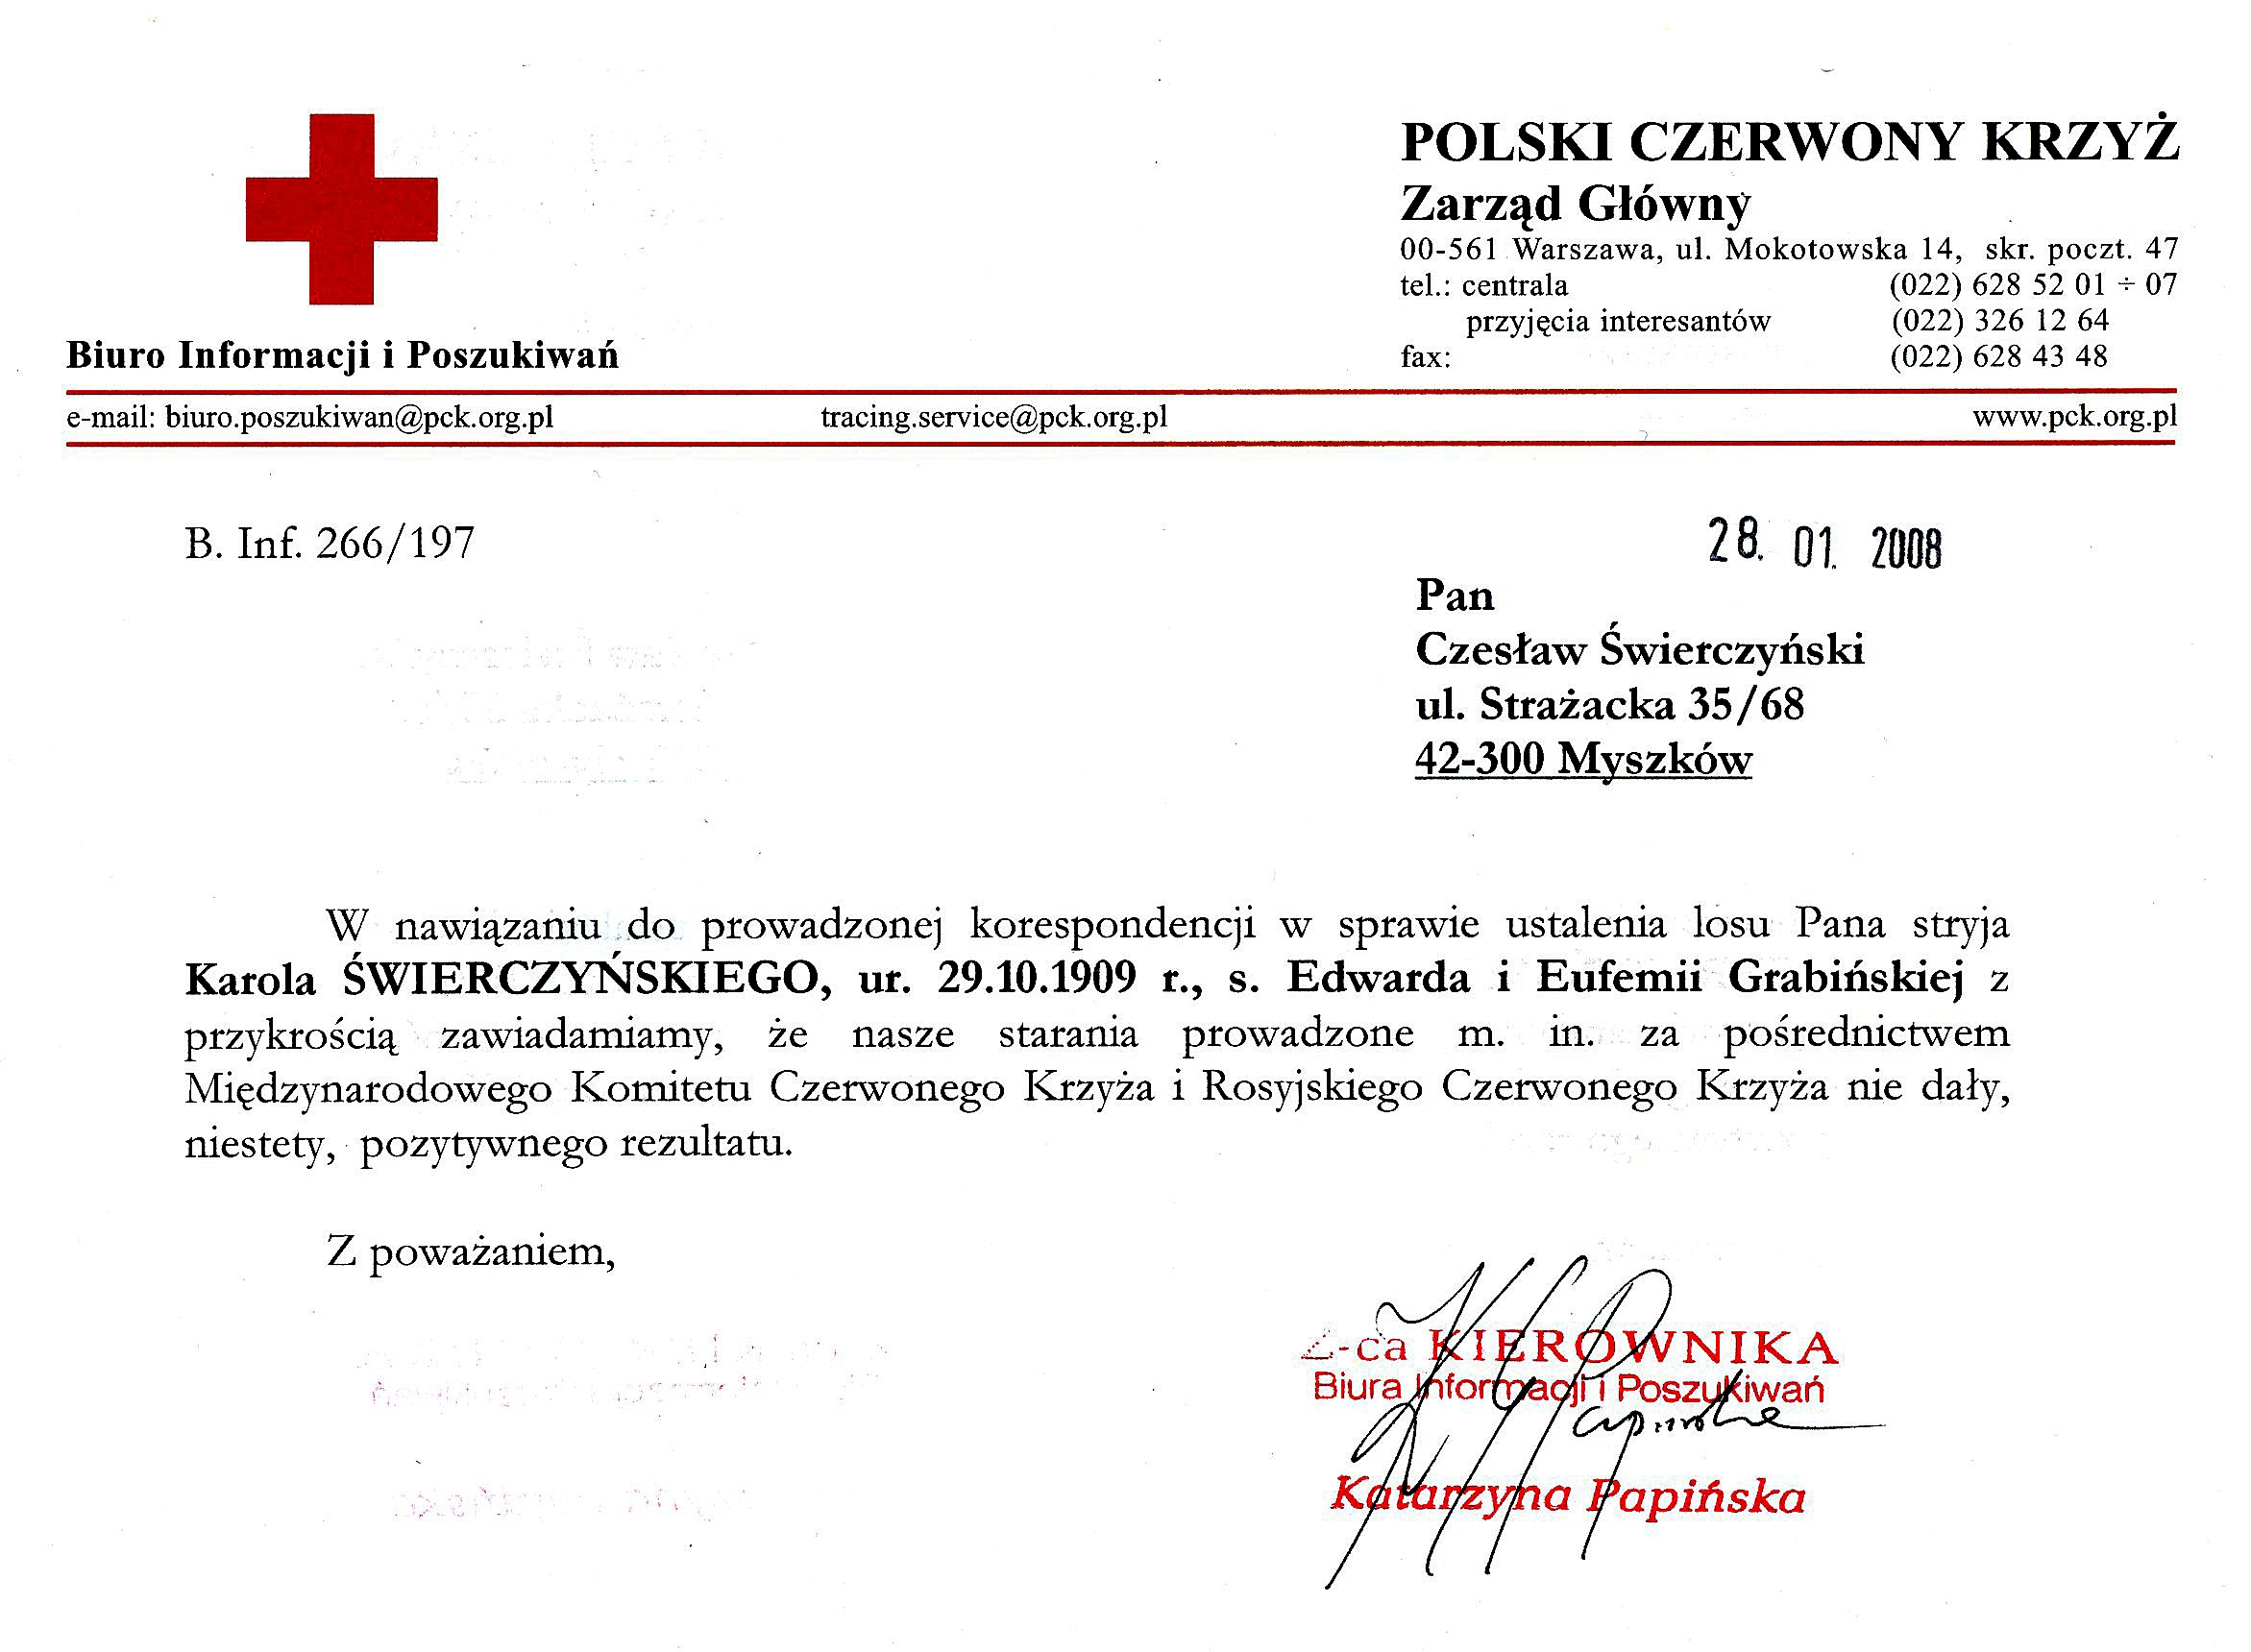
\includegraphics[width=\textwidth]{photo/karol_swierczynski_pck.jpg}
\caption{Oświadczenie PCK w sprawie Karola Świerczyńskiego}
\label{rys:karol_swierczynski_pck}
\end{center}
\end{figure}

Osobiście wysłałem listy do wszystkich znaczących instytucji zajmujących się poszukiwaniem ofiar II wojny światowej. Czas powojenny reżimu komunistycznego nie sprzyjał poszukiwaniom. Natomiast lata od 1956~r. należało wykorzystać na intensywne wynajdywanie śladów, póki żyli żołnierze -- uczestnicy tamtej wrześniowej, tragicznej kampanii. Jego żyjący wówczas bracia niestety nie wykorzystali tej szansy\ldots